\chapter{Implementation}
\label{chap:implementation}

\section{Development Environment}
Describe the development environment, project organization, and configuration needed to reproduce the work.

\section{Key Features}
Present the most important implemented features. For each feature, explain the purpose, the implementation approach, and the result for the user.

\section{User Interface and Demonstration}
Add only the screenshots that help a reader understand a significant workflow. Each screenshot should have a readable caption and a short explanation in the surrounding text.

\begin{figure}[H]
\centering
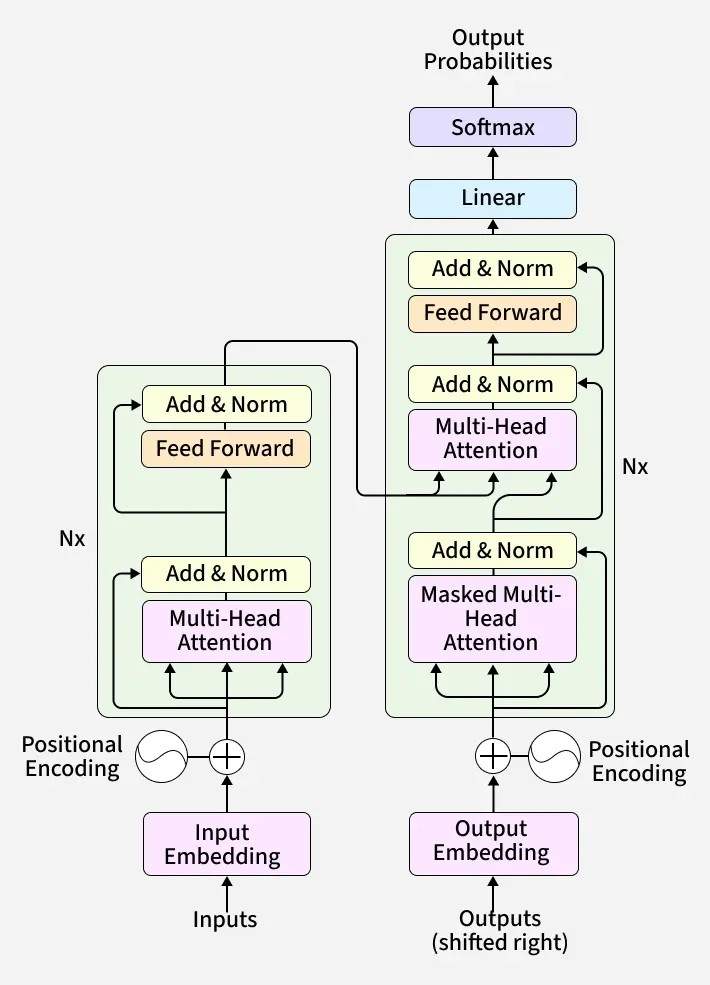
\includegraphics[width=0.78\textwidth]{images/transformers.jpg}
\caption{Example architecture figure. Replace the image and caption with content relevant to your project.}
\label{fig:example-image}
\end{figure}

To insert an image, place it in a folder such as \texttt{Figures/} and replace the placeholder above with:
\begin{verbatim}
\includegraphics[width=0.78\textwidth]{Figures/your-image.png}
\end{verbatim}
Use a clear filename, reference the figure in the text as Figure~\ref{fig:example-image}, and keep only images that support the explanation.

\section{Deployment}
Explain how the solution is delivered or deployed, if this is within the project scope.

\section*{Conclusion}
This chapter shows how the proposed design was translated into a working solution.
